\documentclass[11pt, a4paper]{article}
\usepackage[a4paper, margin=2.2cm]{geometry}
\usepackage[utf8]{inputenc}
\usepackage[T1]{fontenc}
\usepackage{lmodern}
\usepackage{amsmath}
\usepackage{booktabs}
\usepackage{tabularx}
\usepackage{enumitem}
\usepackage{listings}
\usepackage[table]{xcolor}
\usepackage{hyperref}
\usepackage{graphicx}

\definecolor{primaryblue}{HTML}{1468B3}
\definecolor{slateborder}{HTML}{CBD5E1}
\definecolor{codebg}{HTML}{F8FAFC}
\definecolor{headerbg}{HTML}{EFF6FF}

\hypersetup{
    colorlinks=true,
    linkcolor=primaryblue,
    urlcolor=primaryblue
}

\lstset{
    basicstyle=\ttfamily\footnotesize,
    backgroundcolor=\color{codebg},
    frame=single,
    rulecolor=\color{slateborder},
    breaklines=true,
    breakatwhitespace=true,
    showstringspaces=false,
    tabsize=4,
    xleftmargin=4pt,
    xrightmargin=4pt,
    aboveskip=8pt,
    belowskip=8pt
}

\title{\textbf{COSC 3380: Distributed Supermarket \& Banking OLTP Web Application}\\
\large Project Report --- Team 18}
\author{Ramiz Dadabhoy, Mark Gonzalez, Taqib Bhuiyan}
\date{\today}

\begin{document}

\maketitle

\begin{abstract}
This report documents the design, relational schema, distributed transaction processing architecture, and analytical querying capabilities of the Supermarket web application. The system coordinates atomic point of sale checkout operations across two physically separate databases (\texttt{supermarket\_db} and \texttt{bank\_db}) via a custom Two-Phase Commit (2PC) coordinator.
\end{abstract}

\tableofcontents
\newpage

\section{Demo Video Link}
Complete video walkthrough available here:
\begin{itemize}
    \item \textbf{Project Demo Video:} \url{https://streamable.com/mfg4xu}
\end{itemize}

\section{Written Summary of the Web Application}

\subsection{System Architecture}
\begin{enumerate}
    \item \textbf{Front End GUI:} A control panel to simulate user operations. It provides four operational views: \textit{Home / Database} (lifecycle controls and live table previews), \textit{OLTP Simulation} (deterministic integration tests and multi-client concurrent checkout execution), \textit{Analytical Reports} (aggregated sales and low-stock views), and \textit{Transaction History} (chronological audit log with timestamp range filtering).
    \item \textbf{Back End Business Logic:} Exposes REST endpoints \texttt{/api/*} for functionality. It validates inputs, coordinates distributed transactions, and computes subtotals, state sales taxes, and time to execute in ms.
    \item \textbf{Database:} Two independent PostgreSQL connection pools (\texttt{supermarket} and \texttt{bank} managing retail operations and customer/company financial accounts respectively.
\end{enumerate}

\subsection{Distributed Two-Phase Commit (2PC) \& Concurrency Control}
\textit{Note: For realism, we performed additional research to learn and utilize two phase commits, in order to completely separate the Banking \& Supermarket Databases.} \\\\
To enforce all four ACID properties across both databases, \texttt{transactionCoordinator.js} implements a durable Two-Phase Commit (2PC) protocol backed by PostgreSQL prepared transactions (\texttt{PREPARE TRANSACTION}):

\begin{itemize}
    \item \textbf{Lock:} On startup, \texttt{initializeCoordinator()} acquires a PostgreSQL session advisory lock (\texttt{pg\_try\_advisory\_lock(3380, 2001)}) to prevent recovery conflicts and resolves any incomplete transactions recorded in \texttt{distributed\_transactions} before accepting HTTP traffic.
    \item \textbf{Phase 1:} The coordinator records an initial \texttt{ROLLBACK} decision in \texttt{distributed\_transactions}, opens local transactions (\texttt{BEGIN}) on both database pools, executes \texttt{supermarketWork} and \texttt{bankWork}, inserts commit markers into each participant's \texttt{distributed\_participant\_commits} table, and issues \texttt{PREPARE TRANSACTION 'store\_<uuid>'} and \texttt{PREPARE TRANSACTION 'bank\_<uuid>'}.
    \item \textbf{Phase 2:} Once both participants persist their prepared state to Write-Ahead Logs (WAL), the coordinator atomically updates \texttt{decision = 'COMMIT'} in \texttt{distributed\_transactions} and executes \texttt{COMMIT PREPARED} on both databases. If any validation, stock check, or balance check fails during Phase 1, both local transactions are rolled back and the global decision remains \texttt{ROLLBACK}.
    \item \textbf{Deadlock Prevention \& Row-Level Locking:} During concurrent checkout simulations, \texttt{checkoutService.js} sorts requested SKUs lexicographically before executing \texttt{SELECT ... FOR UPDATE OF i} on \texttt{inventory}, ensuring a deterministic global lock acquisition order that prevents circular deadlocks.
\end{itemize}

\section{Entity-Relationship (ER) Diagrams \& Relational Schemas}

\subsection{Database 1: \texttt{supermarket\_db} Conceptual \& Relational Design}
The retail database models multi-branch store operations, state-level tax jurisdictions, aisle-level inventory placement, customer profiles, itemized receipts, and 2PC coordinator logs.

\begin{table}[htbp]
\centering
\caption{Entity and Relationship Summary for \texttt{supermarket\_db}}
\label{tab:supermarket_entities}
\begin{tabularx}{\textwidth}{l l X}
\toprule
\textbf{Relation Name} & \textbf{Primary Key} & \textbf{Attributes \& Foreign Key Constraints} \\
\midrule
\texttt{state\_tax} & \texttt{state} & \texttt{tax\_rate NUMERIC(5,4)} with domain check $0 \le \text{tax\_rate} \le 1$. \\
\texttt{store} & \texttt{store\_id} & \texttt{name, address, city, state, zip}; FK \texttt{state} $\rightarrow$ \texttt{state\_tax(state)}. \\
\texttt{aisle} & \texttt{(store\_id, aisle\_number)} & Weak/identifying entity of \texttt{store}; \texttt{category}; FK \texttt{store\_id} $\rightarrow$ \texttt{store}. \\
\texttt{product} & \texttt{sku} & \texttt{name, price, taxable, by\_weight} with check $\text{price} \ge 0$. \\
\texttt{inventory} & \texttt{(store\_id, sku)} & M:N associative entity linking \texttt{store}, \texttt{product}, and \texttt{aisle}; \texttt{quantity} ($\ge 0$). \\
\texttt{customer} & \texttt{customer\_id} & \texttt{first\_name, last\_name, email, phone}. \\
\texttt{purchase} & \texttt{purchase\_id} & \texttt{store\_id, customer\_id, purchase\_date, total, payment\_method, account\_id}. \\
\texttt{purchase\_item} & \texttt{(purchase\_id, line\_number)} & Weak entity of \texttt{purchase}; \texttt{sku, quantity, unit\_price, tax\_amount}. \\
\texttt{distributed\_transactions} & \texttt{transaction\_id} & \texttt{store\_gid, bank\_gid, decision, completed, created\_at, completed\_at}. \\
\bottomrule
\end{tabularx}
\end{table}

\begin{figure}[htbp]
\centering
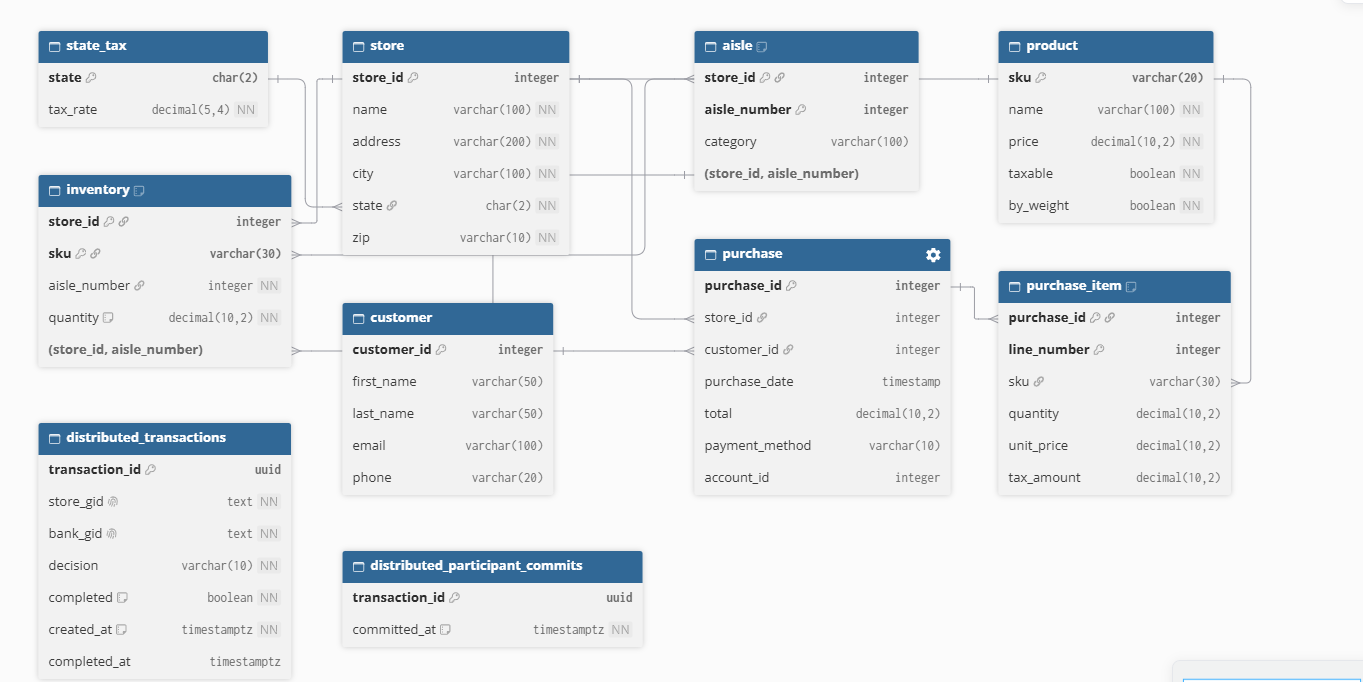
\includegraphics[width=0.95\textwidth]{mainschema.png}
\caption{Entity-Relationship (ER) Structural Diagram for \texttt{supermarket\_db} showing cardinalities and identifying keys.}
\label{fig:er_supermarket}
\end{figure}

\begin{figure}[htbp]
\centering
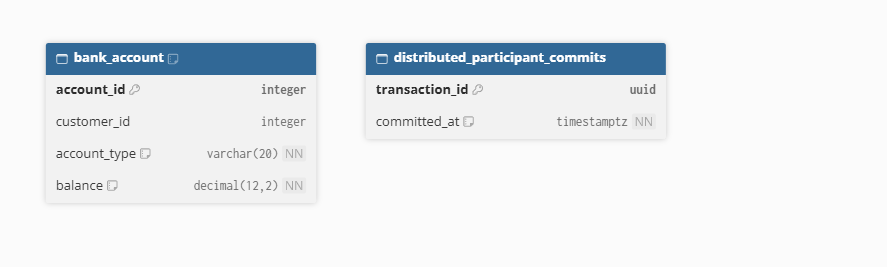
\includegraphics[width=0.85\textwidth]{bankschema.png}
\caption{ER Structural Diagram for \texttt{bank\_db} and its Two-Phase Commit linkage to \texttt{supermarket\_db}.}
\label{fig:er_bank}
\end{figure}

\section{SQL for Distributed Checkout Transactions}
The core OLTP checkout workload executes inside \texttt{processCheckout()} (\texttt{checkoutService.js}) wrapped by \texttt{runDistributedTransaction()} (\texttt{transactionCoordinator.js}). On \texttt{supermarket\_db}, the transaction uses a Common Table Expression (CTE) with \texttt{UNNEST} to join requested SKUs against \texttt{inventory}, \texttt{product}, \texttt{store}, and \texttt{state\_tax}, locking matching inventory rows in sorted SKU order via \texttt{SELECT ... FOR UPDATE OF i} and computing subtotals and state sales taxes in integer cents. It then executes \texttt{INSERT INTO public.purchase ... RETURNING purchase\_id} to create the receipt header, records each line item in \texttt{purchase\_item}, and decrements stock with \texttt{UPDATE public.inventory SET quantity = quantity - \$1}.

For \texttt{CARD} checkouts, the banking participant on \texttt{bank\_db} locks the customer's row via \texttt{SELECT balance FROM public.bank\_account WHERE account\_id = \$1 AND customer\_id = \$2 FOR UPDATE} to verify account ownership and prevent concurrent overdrafts. It then atomically deducts the receipt total using \texttt{UPDATE public.bank\_account SET balance = balance - \$1 WHERE account\_id = \$2 AND customer\_id = \$3 AND balance >= \$1} and transfers the payment to the merchant via \texttt{UPDATE public.bank\_account SET balance = balance + \$1 WHERE account\_type = 'COMPANY'}.

To guarantee cross-database atomicity, both participants insert a tracking row into their local \texttt{distributed\_participant\_commits} table and persist their work via \texttt{PREPARE TRANSACTION 'store\_<uuid>'} and \texttt{PREPARE TRANSACTION 'bank\_<uuid>'}. Once both prepared transactions succeed, the coordinator updates \texttt{decision = 'COMMIT'} in \texttt{distributed\_transactions} and executes \texttt{COMMIT PREPARED} on both databases, or rolls back both branches if any validation or balance check fails.

\section{SQL for Analytical \& Operational Queries}
In addition to OLTP checkouts, the application supports management decision-making and auditing through multi-table joins and aggregate queries across the core tables (\texttt{store}, \texttt{purchase}, \texttt{purchase\_item}, \texttt{product}, \texttt{inventory}, and \texttt{aisle}).

\textbf{Store Sales Summary (\texttt{GET /api/reports/store-sales}):} This query evaluates branch performance by performing a \texttt{LEFT JOIN} from \texttt{public.store} to \texttt{public.purchase} on \texttt{store\_id}, grouping by \texttt{store\_id} and \texttt{name}. Using \texttt{COUNT(p.purchase\_id)} and \texttt{COALESCE(SUM(p.total), 0)}, it computes transaction counts and gross sales while preserving branches with zero purchases, sorting results in descending order of \texttt{total\_sales}.

\textbf{Top-Selling Products (\texttt{GET /api/reports/top-products}):} This query ranks merchandise demand by joining \texttt{public.product} with \texttt{public.purchase\_item} on \texttt{sku} via a \texttt{LEFT JOIN} and grouping by \texttt{sku} and \texttt{name}. It aggregates total units or weight sold with \texttt{COALESCE(SUM(pi.quantity), 0)} and pre-tax revenue with \texttt{COALESCE(SUM(pi.quantity * pi.unit\_price), 0)}, ordering products by \texttt{quantity\_sold DESC}.

\textbf{Low Stock by Aisle (\texttt{GET /api/reports/low-stock}):} This query identifies restocking priorities through a four-way inner join linking \texttt{public.inventory} with \texttt{public.store}, \texttt{public.product}, and \texttt{public.aisle} on \texttt{store\_id}, \texttt{sku}, and \texttt{aisle\_number}. Filtering with \texttt{WHERE i.quantity < 50}, it returns the store name, aisle number, category, SKU, product name, and remaining stock ordered by store, aisle, and lowest quantity.

\textbf{Store Inventory Lookup (\texttt{GET /api/inventory/:storeId}):} This operational query retrieves real-time shelf stock for a specific store branch by joining \texttt{public.inventory} with \texttt{public.product} on \texttt{sku} for a parameterized \texttt{store\_id = \$1}. It projects aisle placement, on-hand quantity, unit price, taxability, and weight flags sorted alphabetically by product name up to 100 rows.

\section{Web References}
The following technical documentation and specifications were referenced during the design and implementation of the application:
\begin{enumerate}
    \item \textbf{PostgreSQL Documentation --- Two-Phase Commit (\texttt{PREPARE TRANSACTION}):} \\
    \url{https://www.postgresql.org/docs/current/sql-prepare-transaction.html}
    \item \textbf{PostgreSQL Documentation --- Explicit Locking (\texttt{SELECT ... FOR UPDATE}):} \\
    \url{https://www.postgresql.org/docs/current/explicit-locking.html}
    \item \textbf{PostgreSQL Documentation --- Advisory Locks (\texttt{pg\_try\_advisory\_lock}):} \\
    \url{https://www.postgresql.org/docs/current/functions-admin.html#FUNCTIONS-ADVISORY-LOCKS}
    \item \textbf{PostgreSQL Documentation --- \texttt{WITH} Queries (Common Table Expressions):} \\
    \url{https://www.postgresql.org/docs/current/queries-with.html}
    \item \textbf{node-postgres (\texttt{pg}) Official Documentation --- Pooling \& Transactions:} \\
    \url{https://node-postgres.com/features/transactions}
    \item \textbf{Express.js Official API Reference (Routing \& Middleware):} \\
    \url{https://expressjs.com/en/4x/api.html}
    \item \textbf{Node.js Documentation --- \texttt{crypto.randomUUID()} \& High-Resolution Timing:} \\
    \url{https://nodejs.org/api/crypto.html#cryptorandomuuidoptions}
    \item \textbf{MDN Web Docs --- Fetch API \& \texttt{AbortController} (Concurrent Request Cancellation):} \\
    \url{https://developer.mozilla.org/en-US/docs/Web/API/AbortController}
    \item \textbf{jQuery API Documentation --- DOM Manipulation \& Event Handling:} \\
    \url{https://api.jquery.com/}
    \item \textbf{Course Textbook Reference:} R. Elmasri and S. B. Navathe, \textit{Fundamentals of Database Systems}, 6th ed., Addison-Wesley, 2011 (Chapters 7, 13, 21, and 22).
\end{enumerate}

\end{document}